\section{Fundamentals and Related Work} \label{fundamentals}

\subsection{From Probabilistic Language Models to modeling Evolution Theory} \label{fundamentalsA}

A probabilistic language model tries to approximate the probability distribution 

\begin{equation}
	P(w_1, ..., w_n) = \Pi_{t=1}^{n} P(w_t | w_1, ..., w_{t-1})
\end{equation}

with $w_t$ being a word at position (timestamp) $t$ in a sentence of length $n$. To build language models \acp{RNN} were used to model such probability distributions. 

\begin{figure}[ht]
	\centering
	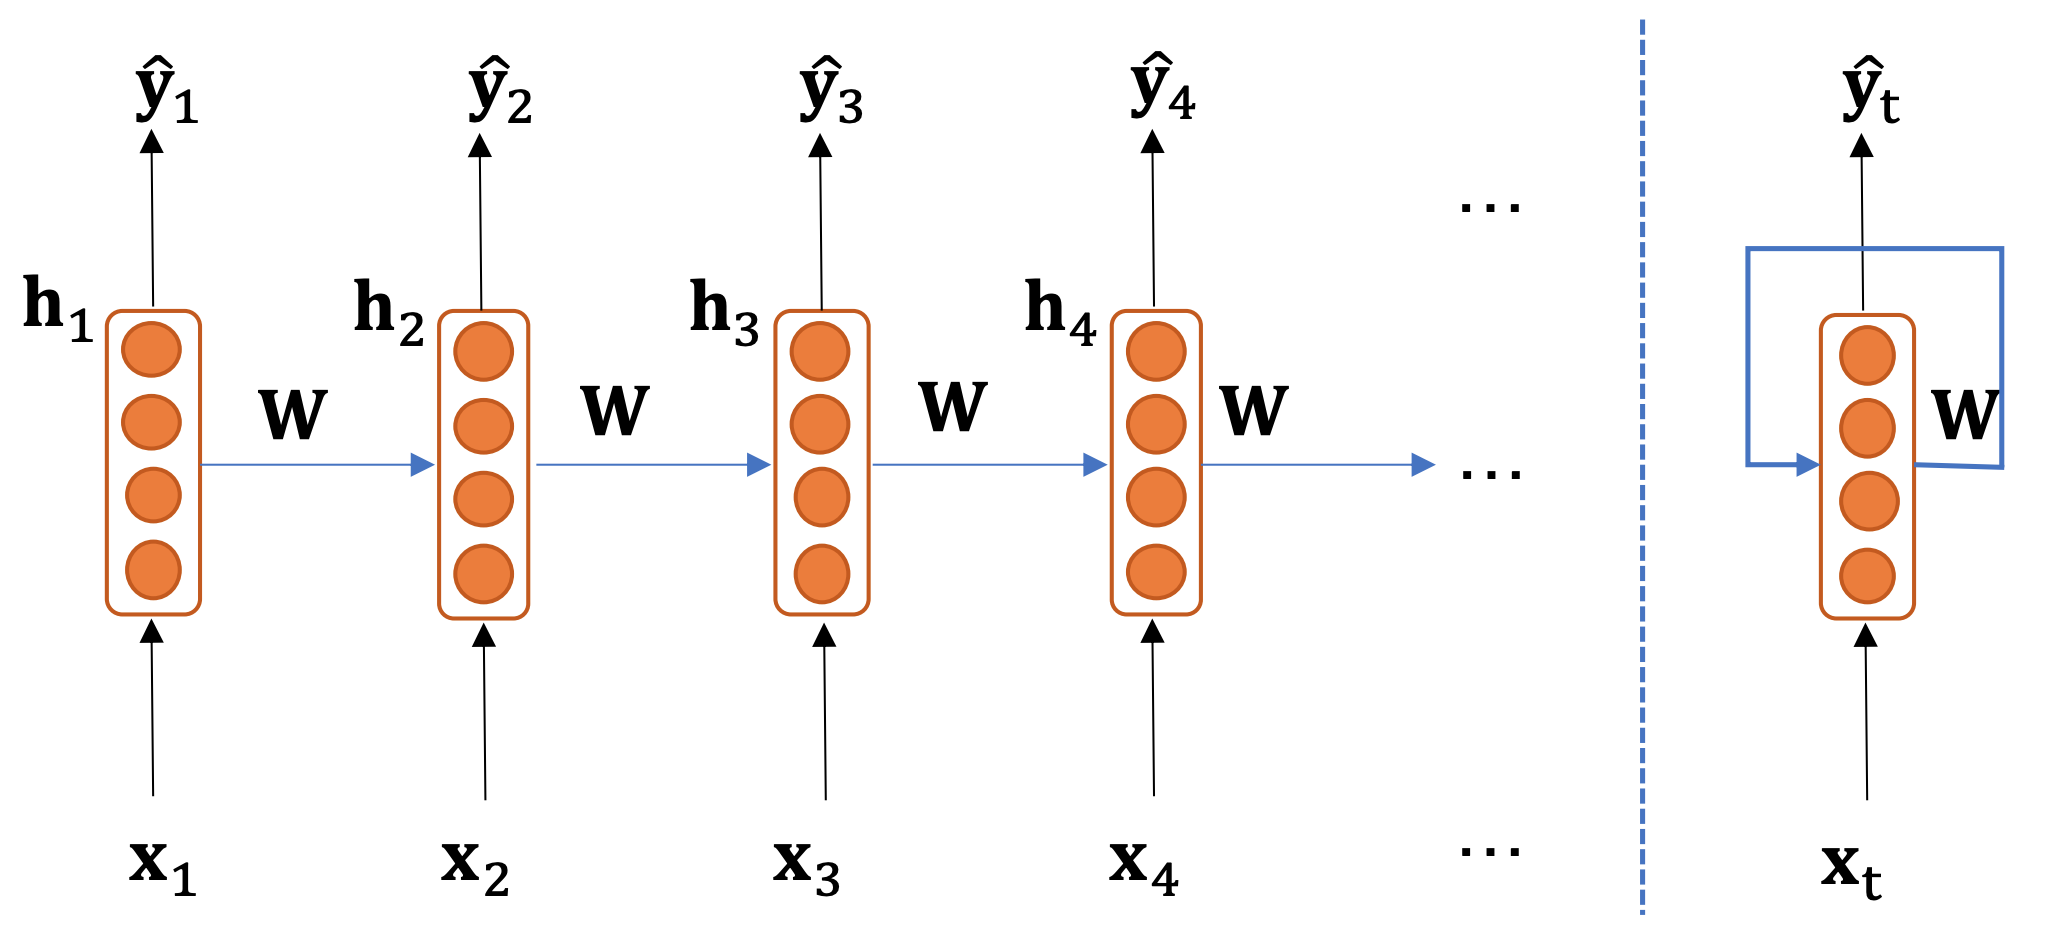
\includegraphics[width=1.0\linewidth]{figures/rnn_architecture.png}
	\caption{Architecture of a conventional \ac{RNN} \cite{Gertz2020}}
	\label{rnn_architecture}
\end{figure}

At each time step $t$ it outputs a probability distribution $P(w_t | w_1, ..., w_{t-1})$ given the words read so far in the current instance (see \autoref{rnn_architecture}). Words are read as a vectorized numerical representation, often given by pretrained so-called word embeddings $x_t$ which are lower dimensional and more semantically-enriched compared to simple one-hot encodings. One then calculates the hidden state $h_t$ by

\begin{equation}
	h_t = f(W^{(h)} h_{t-1} + W^{(x)} x_t + b_1)
\end{equation}

and the corresponding output porbability distribution by 

\begin{equation}
	\hat{y}_t = softmax(U^{(h)} h_t + b_2).
\end{equation}

The applied weight matrix is always the same for each time step $t$ giving the \ac{RNN} its name. One can therefore simplify the unrolled \ac{RNN} architecture on the left side of \autoref{rnn_architecture} to the one on the right, where the hidden state is continuously passed as an input to the next time step. To achieve a better convergence behavior during training, one can also provide the expected hidden state of time step $t-1$ instead of using the predicted hidden state, which is called teacher forcing. \acp{RNN} are able to process input of arbitrary length and are by their recurrent character capable to use information from previous time steps. Unfortunately, they are vulerable to vanishing and exploding gradient problems. \ac{LSTM} is a special \ac{RNN} architecture that solves such vulnerabilities by owning a separate long-term cell state besides a short-term hidden state and is introduces in \autoref{fundamentalsE}. It is able to preserve information over many time steps. \cite{Gertz2020}

\begin{figure}[ht]
	\centering
	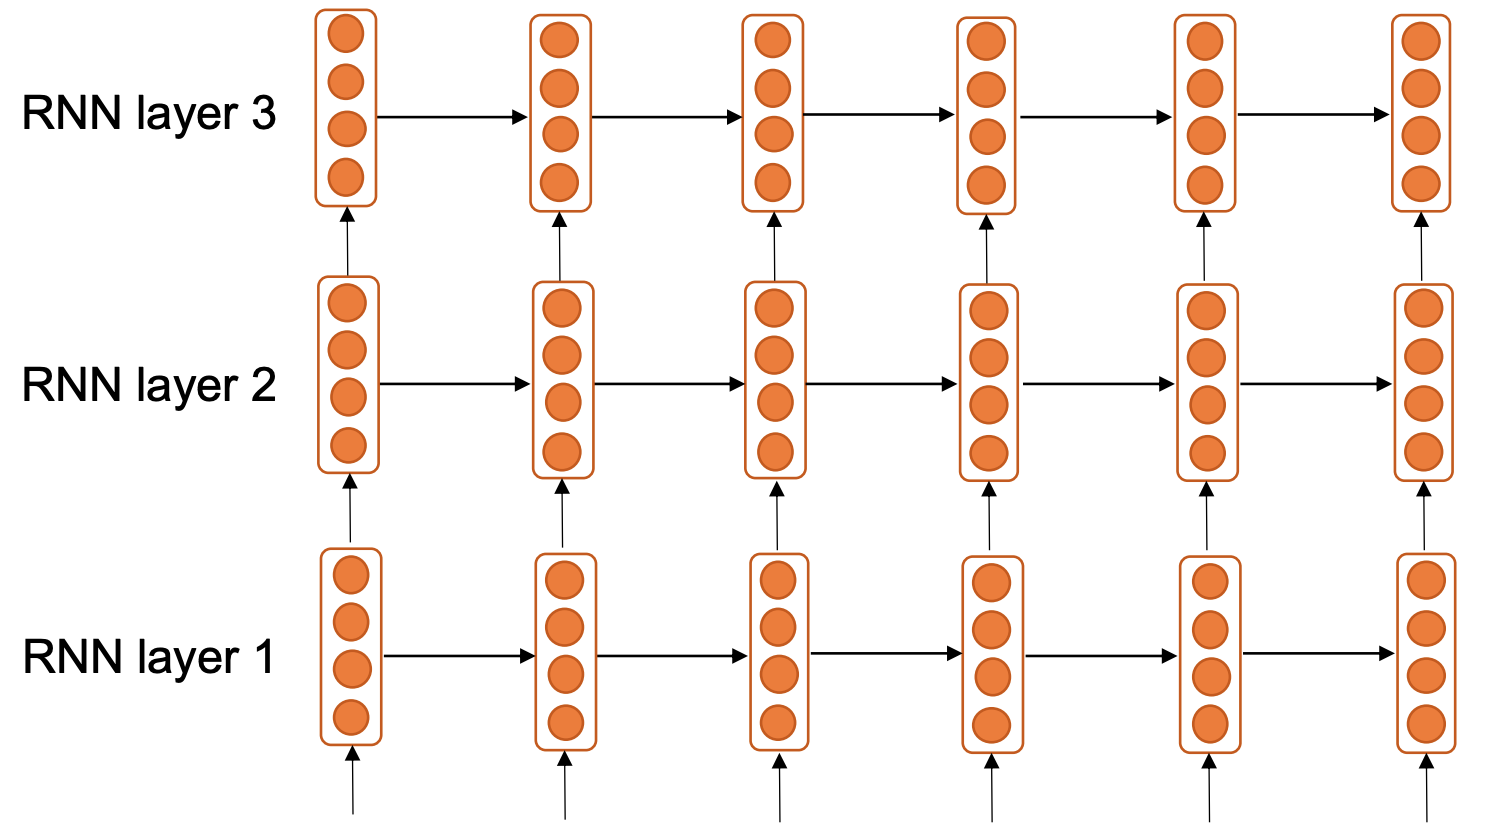
\includegraphics[width=0.8\linewidth]{figures/multi_layer_rnn.png}
	\caption{Architecture of a multi-layer  \ac{RNN} \cite{Gertz2020}}
	\label{multi_layer_rnn}
\end{figure}

One can also use two \acp{RNN}, one traversing a sentence from left to right and another one vice versa, with two different weight matrices to model the probability distribution bidirectionally. One therefore simply concatenates the hidden states of each \ac{RNN} before applying the the weight matrix $U$ and the $softmax()$ function. Also multi-layer \acs{RNN} can be utilized to generate higher-order features (hidden states) for the prediction task (see \autoref{multi_layer_rnn}). \cite{Gertz2020}

The \acp{RNN} or even better \acp{LSTM} architectures used for probabilistic language modeling can be reused in a more complex domain called sequence to sequence modeling for neural machine translation from one language to another. Here one first tries to learn a fixed-dimensional input representation from an input sequence using an encoder architecture based on an \ac{LSTM}. The so-called context vector is then decoded by a second \ac{LSTM} into a new sequence of words preserving the grammar but owning a different meaning. \cite{Sutskever2014}

Sequence to sequence models are introduced together with the \ac{LSTM} architecture in \autoref{fundamentalsE}. Here the connection to evolution theory can be drawn. \ac{RNA} sequences made of a concatenation of nucleotides \footnote{We restrict the representation of nucleotides solely to their nucleobases parts consisting of the distinct nucleobases guanine, adenine, cytosine and thymine. We therefore do not include the phosphate group and the five-carbon sugar components.} can be represented textually using the FASTA format. A sequence to sequence model can then transferably be applied in the domain of \ac{RNA} sequences to model how \ac{RNA}-based viruses change their structure to avoid the detection by the human immune system but still to preserve their infectivity and evolutionary fitness \cite{Hie2021}. 

\subsection{GISAID EpiFlu Data Platform} \label{fundamentalsB}

\subsection{Domain-Specific Methodologies to create Evolutionary  Datasets for Mutation Prediction} \label{fundamentalsC}

\subsection{Previous Work on Mutation Prediction} \label{fundamentalsD}

Even before the rise of Covid-19 there had been studies trying to predict mutations of RNA viruses. In the collection of \cite{Wu2007, Yan2007, Wu2008} the authors predict the mutation positions in hemagglutinins from influenza A virus using logistic regression and plain neural networks and then use the resulting amino acid mutating probabilities to derive possible mutated amnio acids. The same approach is further used for H5N1 neuraminidase proteins. 

\cite{Salama2016} proved that nucleotides in an RNA sequence can change based on their local neighborhood. Neural networks are used to predict new strains of the Newcastle virus and subsequently a rough set theory based algorithm is introduced to extract the according point mutation patterns. 

\cite{Mohamed2021} uses a more modern sequence to sequence approach based on \acp{LSTM} to learn nucleotide mutations between time-series species of H1N1 Influenza virus and the Newcastle virus as mutations can also be influenced by long-distance relations of amino acids. Therefore one hot-encoded RNA sequences of a parent generation preprocessed to words is given as an input and the output is the predicted offspring generation evaluated by accuracy to the compared true offspring generation. The achieved accuracy in this paper is questionably high with 98.9\% on the H1N1 Influenza virus and 96.9\% on the Newcastle virus, possibly because of overfitting to the few 4.609 samples for H1N1 Influenza virus and only 83 for the Newcastle virus. Our approach therefore tries to increase the number of samples available for training when building the dataset. 

Our approach will neither use any of the just mentioned architectures, but uses a Transformer based architecture coupled with a GAN-style training architecture. Nevertheless a short introduction into sequence to sequence models and the underlying long short-term memory components shall be given to better point out our architectural decisions . 

\subsection{Sequence to Sequence Models based on Long Short-Term Memory} \label{fundamentalsE}

% Figure Seq2Seq

The original \ac{LSTM} unit was introduced in \cite{Hochreiter1997} and can be used for language modeling instead of using plain \acp{RNN} to prevent running into vanishing or exploding gradient problems \cite{Sundermeyer2012}. The architecture of an \ac{LSTM} is shwon in the following figure:

\begin{figure}[ht]
	\centering
	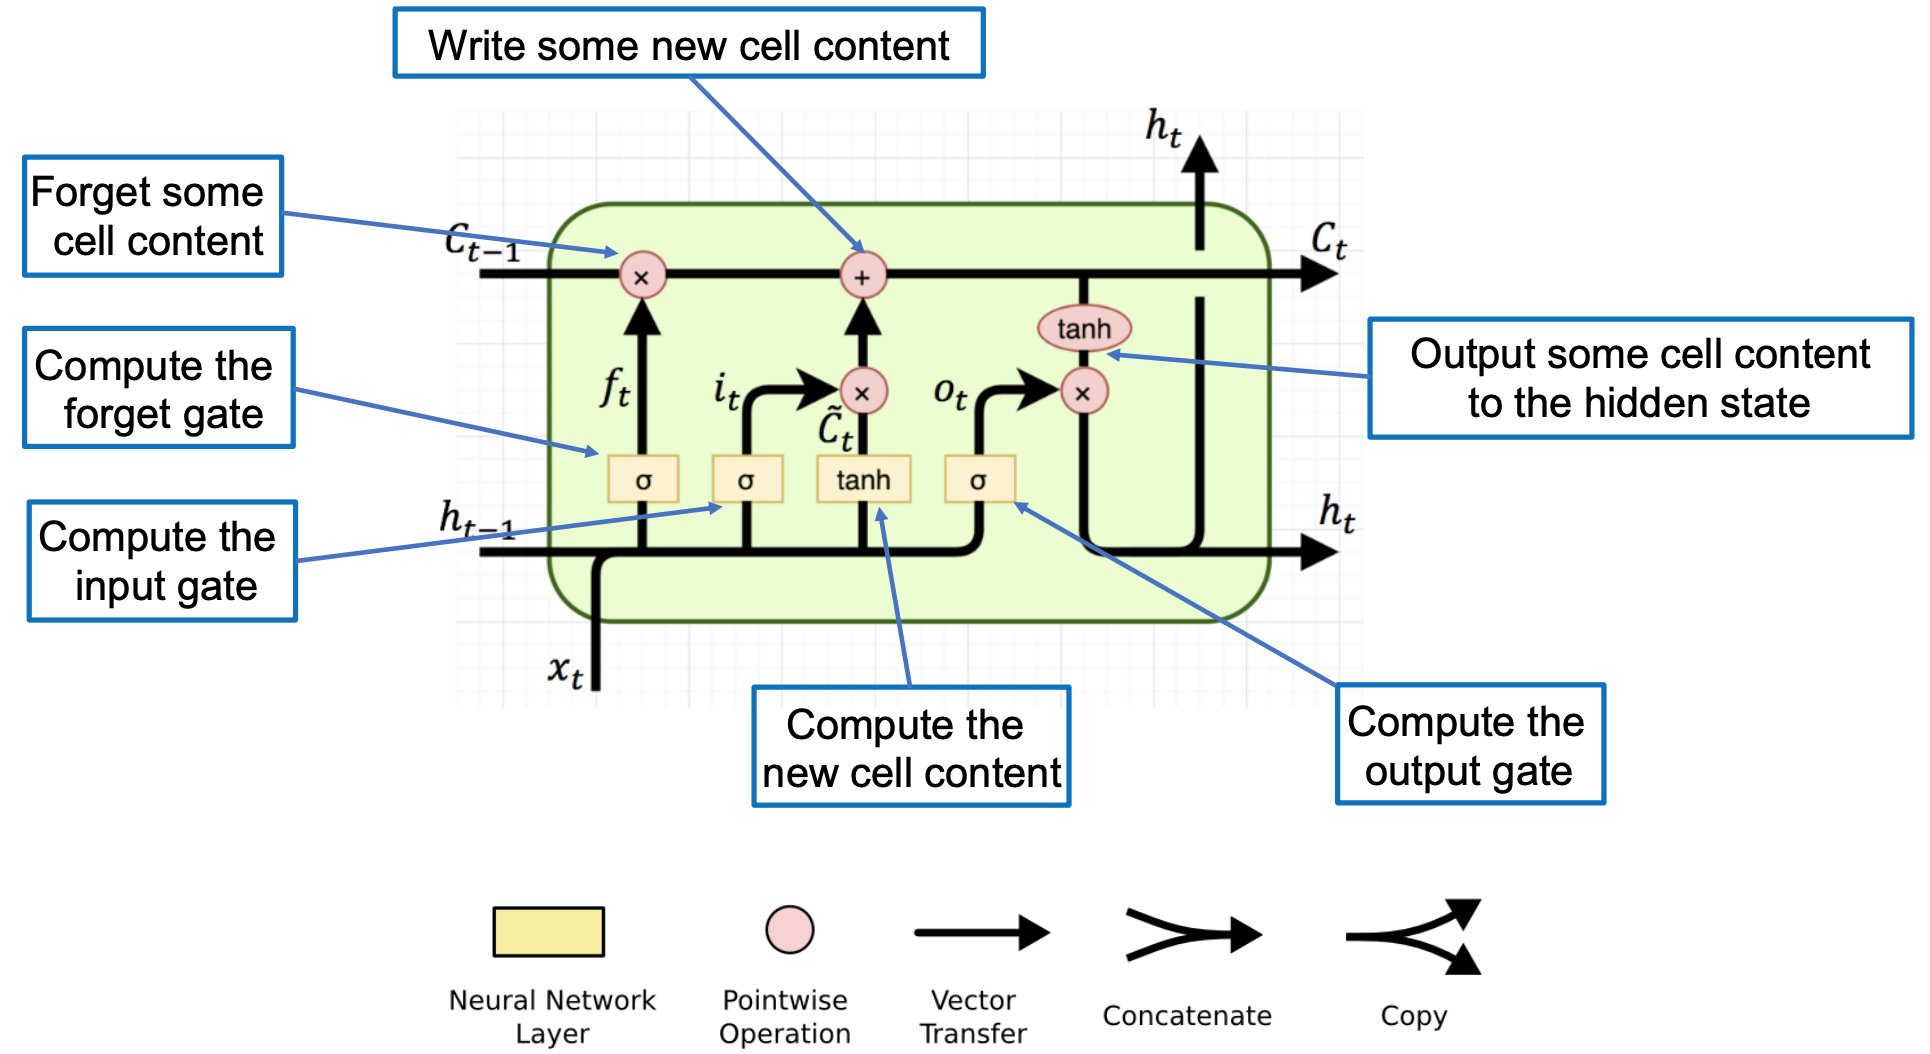
\includegraphics[width=0.8\linewidth]{figures/lstm_architecture.png}
	\caption{Architecture of an \ac{LSTM} \cite{Gertz2020}}
	\label{lstm_architecture}
\end{figure}

It consists of a hidden state $h_t$ and an additional cell state $c_t$. The cell state stores long-term information and is used to derive a new hidden state. Information flows through three different gates inside the \ac{LSTM}. The forget gate is used to control which parts of the cell state are potentially carried on to the next time step, the input gate is responsible to decide which parts of the cell state should be updated and the output gate determines what is being passed on as the new hidden state. All three gates and depend on the previous hidden state and the current input. They provide factors limited to the interval [0,1] by the sigmoid function and are multiplied with the cell state, the changes to be added to the cell state and the new hidden state derived from the cell state. Through the cell state an \ac{LSTM} therefore makes it possible to capture long-distance dependencies. \cite{Gertz2020}

\cite{Sutskever2014} introduced sequence to sequence learning following a multi-layer encoder-decoder style model architecture. One layer consists of one \ac{LSTM} that is used as an encoder to learn a large fixed-dimensional vector representation of a size-unrestricted input sequence called the context vector. This vector consists of the last cell and hidden state of the encoder and incorporates the structure of the input sequence helping the followig decoder \ac{LSTM} to provide qualitative predictions for the output sequence. The second \ac{LSTM} therefore serves as a beam search\footnote{Do not choose the most probable word but the $B$ most likely word hypothesis and pass them to the next time step in the \ac{LSTM}. To avoid combinatorial explosion limit the beam depth size.} decoder to map the context vector to a corresponding output sequence whose length does not need to match with the length of the input sequence. The output probabiity distribution is therefore given by the equation

\begin{equation}
	p(y_1, ..., y_{T'} | x_1, ..., x_{T}) = \Pi_{t=1}^{T'} p(y_t | v, y_1, ..., y_{t-1})
\end{equation}

with $v$ being the context vector. Using an \ac{LSTM} is prefered over a normal \ac{RNN} as it is used to capture the long range temporal dependencies of the input data. The encoder-decoder architecture uses four layers in total partitioned onto four \acp{GPU}. A corpus of 160k words for the input sequence and another one of 80k words for the target sequence was used to create the word embeddings of dimension 1000. Unknown words were replaced by a \textit{UNK} token. The sequence to sequence model approach was evaluated for neural machine translation and reached a 34.81 BLEU score. One finding during training was that reversing the input sequence introduces many short term dependencies as the minimal time lag of the problem is reduced making optimization easier. \cite{Sutskever2014}

\subsection{Applying Generative Adversarial Networks} \label{fundamentalsF}

\begin{itemize}
	\item Covid-Paper: \url{https://arxiv.org/pdf/2008.11790.pdf}
\end{itemize}


\subsection{Transformer and Attention Mechanism} \label{fundamentalsG}

- Attention allows the model to focus on the relevant parts of the input sequence as needed
- Encoder passes all hidden states to the decoder
- Decoder generated a context vector for each time step from all the encoder hidden states

\begin{itemize}
	\item Improvement: \url{https://arxiv.org/abs/1706.03762}
\end{itemize}


\subsection{Other Techniques} \label{fundamentalsH}

\begin{itemize}
	\item NNs/SVMs: \url{https://bsb-eurasipjournals.springeropen.com/articles/10.1186/s13637-016-0042-0}
	\item BiLSTM: \url{https://science.sciencemag.org/content/371/6526/284}
\end{itemize}


\newpage
